\documentclass[10pt]{article}

% Manage page layout
\usepackage[margin=2.5cm, includefoot, footskip=30pt]{geometry}
\pagestyle{plain}
\setlength{\parindent}{0em}
\setlength{\parskip}{1em}
\renewcommand{\baselinestretch}{1}

%%%%%%%PACKAGES HERE%%%%%%%
\usepackage{tikz}
\usepackage{amsmath}
\usepackage{amssymb}
\usepackage{graphicx}
\usepackage{subcaption}
\usepackage{standalone}
\usepackage{booktabs}
\usepackage{algorithm, setspace}
\usepackage[noend]{algpseudocode}

\makeatletter
\def\BState{\State\hskip-\ALG@thistlm}
\makeatother

\newcommand{\R}{\mathbb{R}}
\newtheorem{theorem}{Theorem}
\usetikzlibrary{decorations.pathmorphing, decorations.pathreplacing, angles,
                quotes, calc, er, positioning}

\newtheorem{lemma}[theorem]{Lemma}
\def\arraystretch{1.5}
%%%%%%%%%%%%%%%%%%%%%%%%%%%
\title{Memory size in the Prisoner's Dilemma}
\author{Nikoleta E. Glynatsi \and Vincent Knight}
\date{}

\begin{document}

\maketitle

\begin{abstract}

In this manuscript we build upon a framework provided in 1989 for the study of
these strategies and identify the best responses of memory one players. The aim
of this work is to show the limitations of memory one strategies in multi-opponent
interactions. A number of theoretic results are presented.
%TODO: Expand when we get results
\end{abstract}

\section{Introduction}\label{section:introduction}

The Prisoner's Dilemma (PD) is a two player person game used in understanding the
evolution of co-operative behaviour. Each player can choose between cooperation
(C) and defection (D). The decisions are made simultaneously and independently.
The normal form representation of the game is given by:

\begin{equation}\label{equ:pd_definition}
    S_p = \begin{pmatrix}
    R & S  \\
    T & P
    \end{pmatrix} \quad
    S_q = \begin{pmatrix}
        R & T  \\
        S & P
        \end{pmatrix}
\end{equation}

where \(S_p\) represents the utilities of the first player and \(S_q\) the utilities
of the second player. The payoffs, \((R, P, S, T)\), are constrained by equations
(\ref{eq:pd_constrain_one}) and~(\ref{eq:pd_constrain_two}). Constrain
(\ref{eq:pd_constrain_one}) ensures that defection dominates cooperation and
constrain (\ref{eq:pd_constrain_two}) ensures that there is a dilemma. Because
the sum of the utilities for both players is better when both choose cooperation.
The most common values used in the literature are \((3, 1, 0, 5)\)~\cite{Axelrod1981}.

\begin{equation}\label{eq:pd_constrain_one}
    T > R > P > S 
\end{equation}

\begin{equation}\label{eq:pd_constrain_two}
    2R > T + S
\end{equation}

The PD is a one shot game, however it is commonly studied in a manner where the
history of the interactions matters. The repeated form of the game is called the
Iterated Prisoner's Dilemma (IPD) and in the 1980s following the work of
\cite{Axelrod1980a, Axelrod1980b} it attracted the attention of the scientific
community.

In~\cite{Axelrod1980a} and~\cite{Axelrod1980b}, the first well known computer
tournaments of the IPD were performed. A total of 13 and 63 strategies were submitted
in computer code and competed against each other in a round robin tournament.
All contestants competed against each other, themselves and random strategy and the
winner was decided on the average score a strategy achieved and not in the number of wins.
The strategies were allowed access to the full history of each match. The history
included the previous moves of both the player and the opponent. How many turns of history
that a strategy would use, the memory size, was left to the creator of the strategy to
decide.

The winning strategy of both tournaments was a strategy called Tit for Tat. Tit for Tat
is a strategy which starts by cooperating and then mimics the last move of
it's opponent. This is a strategy which makes use of the previous move of the opponent
only and it's called a reactive strategy. Reactive strategies have been used
to explore best behaviour in the IPD and a framework for studying such strategies
was introduced in~\cite{Nowak1989}. This was later used to introduce other
reactive strategies such as Generous Tit For Tat~\cite{Nowak1990}.

Reactive strategies are a subset of memory one strategies. Memory one strategies
similarly are only concern with the previous turn. However, they take into consideration
both players' recent moves to decide on an action. Several successful memory one
strategies are found in literature, for example Pavlov~\cite{Nowak1993}.

A well known set of memory on strategies were introduced in~\cite{Press2012}
called zero determinant (ZD) strategies. The ZD strategies, manage to force a linear
relationship between the score of the strategy and the opponent. The authors showed
that ZD strategies were a set of strategies that could dominate any evolutionary
opponent, in pairwise interactions. ZD strategies were dominating using a single
size memory and authors questioned the usefulness of memory in the IPD.

The ZD strategies tracked a lot of attention. It was stated that
``Press and Dyson have fundamentally changed the viewpoint on the Prisoner's
Dilemma''~\cite{Stewart2012}. In~\cite{Stewart2012}, the Axelrod's
tournament have been re-run including ZD strategies and a new set of ZD
strategies the Generous ZD.

Even so, ZD and memory one strategies have also received criticism. In~\cite{Harper2015},
the `memory of a strategy does not matter' statement was questioned. A set of more
complex strategies, strategies that take in account the entire history set of the
game, were trained and proven to be more robust than ZD strategies.

\subsection{The Problem}

In this manuscript we explore the size of memory for strategies of IPD.%TODO: expand when we know the results

The purpose of this work is to consider a given memory one strategy 
in a similar fashion to~\cite{Press2012}. However whilst~\cite{Press2012} found
a way for a player to manipulate an opponent, this work will consider an
optimisation approach to identify the best response to that opponent.
In essence the aim is to produce a compact method of identifying the best memory
one strategy against a given opponent.

In the second part of this manuscript we explore the limitation of these best response
strategies. This is achieved by comparing the performance of an optimal
memory one strategy, for a given environment, with the performance of a more complex
strategy. The type of complex strategy used is described in depth in the
following Sections. Keep in mind, that the complex strategies used here has a memory
greater than one and it keeps track of the initial move.

\section{Methodology}

In~\cite{Nowak1989} a framework was introduced to study the interactions of memory
one strategies modelled as a stochastic process. The work~\cite{Press2012} of is
also build upon at manuscript. There it is stated that if a strategy
is concerned with only the outcome of a single turn then there are four possible `states'
the strategy could be in. These are \(CC, CD, DC,CC\). A memory one strategy is denoted
by the probabilities of cooperating after each of these states,
\(p=(p_1, p_2, p_3, p_4) \in \R_{[0,1]} ^ 4\). A diagrammatic representation of
such strategy is given in Figure~\ref{fig:diagram_mem_one}.

\begin{figure}
    \centering
    \begin{subfigure}{0.45\textwidth}
        \centering
        \includestandalone[width=.65\textwidth]{tex/states}
        \subcaption{Diagrammatic representation of a memory one strategy.}
        \label{fig:diagram_mem_one}
    \end{subfigure}
    \begin{subfigure}{0.45\textwidth}
        \centering
        \includestandalone[width=.88\textwidth]{tex/markov_chain}
        \subcaption{Markov chain on a PD game.}
        \label{fig:markov_chain}
    \end{subfigure}
\end{figure}

Moreover, if two players are moving from state to state using the transition
probabilities, this can be modelled as a Markov process of four states, shown by
Figure~\ref{fig:markov_chain}. The transition matrix \(M\) of Figure~\ref{fig:markov_chain}
is defined as,

\begin{equation}\label{eq:m_matrix}
    M = \left[\begin{matrix}p_{1} q_{1} & p_{1} \left(- q_{1} + 1\right) & q_{1} \left(- p_{1} + 1\right) & \left(- p_{1} + 1\right) \left(- q_{1} + 1\right)\\p_{2} q_{3} & p_{2} \left(- q_{3} + 1\right) & q_{3} \left(- p_{2} + 1\right) & \left(- p_{2} + 1\right) \left(- q_{3} + 1\right)\\p_{3} q_{2} & p_{3} \left(- q_{2} + 1\right) & q_{2} \left(- p_{3} + 1\right) & \left(- p_{3} + 1\right) \left(- q_{2} + 1\right)\\p_{4} q_{4} & p_{4} \left(- q_{4} + 1\right) & q_{4} \left(- p_{4} + 1\right) & \left(- p_{4} + 1\right) \left(- q_{4} + 1\right)\end{matrix}\right].
\end{equation}

where the vector of the stationary probabilities of is \(v\)(given in the Appendix). %TODO include Appendix
Combining the stationary vector \(v\) with the payoff matrices\ref{equ:pd_definition}
allow us to retrieve the expected outcome for each player. Thus, the utility for
player \(p\) against \(q\), denoted as \(u_q(p)\), can defined by,

\begin{equation}\label{eq:press_dyson_utility}
    u_q(p) = v \times S_p.
\end{equation}

The analytical formulation gives the advantage of time. That is because the 
payoffs of a match between two opponents are now retrievable without 
simulating the actual match itself. This analytical formulation will be used
hereupon and it will will allow us to study best responses in an analytical way.

Though this formulation, which was described in 1989~\cite{Nowak1989}, have been
used in several different works not many insights have been given for form of \(u_q(p)\).
Here we present one of our first results which concerns the form \(u_q(p)\). That is
that \(u_q(p)\) is given by a ratio of two quadratic forms, as presented
by Theorem~\ref{theorem:quadratic_form_u}.

\begin{theorem}\label{theorem:quadratic_form_u}
    The expected utility of a memory one strategy \(p\in\mathbb{R}_{[0,1]}^4\)
    against a memory one opponent strategy \(q\in\mathbb{R}_{[0,1]}^4\), denoted
    as \(u_q(p)\), can be written as a ratio of two quadratic forms:

    \begin{equation}\label{eq:optimisation_quadratic}
    u_q(p) = \frac{\frac{1}{2}pQp^T + cp + a}
                {\frac{1}{2}p\bar{Q}p^T + \bar{c}p + \bar{a}}, 
    \end{equation}
    where \(Q, \bar{Q}\) \(4 \times 4\) matrices defined by the transition
    probabilities of the opponent \(q_1, q_2, q_3, q_4\) as follows:
    
    \begin{center}
    \begin{equation}
    \resizebox{0.9\linewidth}{!}{\arraycolsep=2.5pt%
    \boldmath\(
    Q = \left[\begin{matrix}0 & 5 q_{4} \left(q_{1} - q_{3}\right) & - q_{4} \left(q_{1} - q_{2}\right) & \left(q_{1} - q_{4}\right) \left(q_{2} - 5 q_{3} - 1\right)\\5 q_{4} \left(q_{1} - q_{3}\right) & 0 & - 3 q_{4} \left(q_{2} - q_{3}\right) & \left(q_{3} - q_{4}\right) \left(5 q_{1} - 3 q_{2} - 2\right)\\- q_{4} \left(q_{1} - q_{2}\right) & - 3 q_{4} \left(q_{2} - q_{3}\right) & 0 & - \left(q_{2} - q_{4}\right) \left(q_{1} - 3 q_{3} - 1\right)\\\left(q_{1} - q_{4}\right) \left(q_{2} - 5 q_{3} - 1\right) & \left(q_{3} - q_{4}\right) \left(5 q_{1} - 3 q_{2} - 2\right) & - \left(q_{2} - q_{4}\right) \left(q_{1} - 3 q_{3} - 1\right) & 0\end{matrix}\right]\)},
    \end{equation}
    \begin{equation}\label{eq:q_bar_matrix}
    \resizebox{0.8\linewidth}{!}{\arraycolsep=2.5pt%
    \boldmath\(
    \bar{Q} =  \left[\begin{matrix}0 & - \left(q_{1} - q_{3}\right) \left(q_{2} - q_{4} - 1\right) & \left(q_{1} - q_{2}\right) \left(q_{3} - q_{4}\right) & \left(q_{1} - q_{4}\right) \left(q_{2} - q_{3} - 1\right)\\- \left(q_{1} - q_{3}\right) \left(q_{2} - q_{4} - 1\right) & 0 & \left(q_{2} - q_{3}\right) \left(q_{1} - q_{4} - 1\right) & \left(q_{1} - q_{2}\right) \left(q_{3} - q_{4}\right)\\\left(q_{1} - q_{2}\right) \left(q_{3} - q_{4}\right) & \left(q_{2} - q_{3}\right) \left(q_{1} - q_{4} - 1\right) & 0 & - \left(q_{2} - q_{4}\right) \left(q_{1} - q_{3} - 1\right)\\\left(q_{1} - q_{4}\right) \left(q_{2} - q_{3} - 1\right) & \left(q_{1} - q_{2}\right) \left(q_{3} - q_{4}\right) & - \left(q_{2} - q_{4}\right) \left(q_{1} - q_{3} - 1\right) & 0\end{matrix}\right]\)}.
    \end{equation}
    \end{center}
    
    \(c \text{ and } \bar{c}\), are \(4 \times 1\) vectors defined by:
    
    \begin{equation}\label{eq:q_matrix_numerator}
    \resizebox{0.3\linewidth}{!}{\arraycolsep=2.5pt%
    \boldmath\(c = \left[\begin{matrix}- 5 q_{1} q_{4}\\5 q_{4} \left(q_{3} - 1\right)\\q_{4} \left(2 q_{2} + 1\right)\\5 q_{1} q_{4} - 2 q_{2} q_{4} - q_{2} - 5 q_{3} q_{4} + 5 q_{3} - 3 q_{4} + 1\end{matrix}\right]\),}
    \end{equation}
    \begin{equation}\label{eq:q_matrix_denominator}
    \resizebox{0.3\linewidth}{!}{\arraycolsep=2.5pt%
    \boldmath\(\bar{c} = \left[\begin{matrix}q_{1} \left(q_{2} - q_{4} - 1\right)\\- \left(q_{3} - 1\right) \left(q_{2} - q_{4} - 1\right)\\- q_{1} q_{2} + q_{2} q_{3} + q_{2} - q_{3} + q_{4}\\q_{1} q_{4} - q_{2} - q_{3} q_{4} + q_{3} - q_{4} + 1\end{matrix}\right]\).
    }
    \end{equation}
    
    Finally, \(a = 5 q_{4}\) and 
    \(\bar{a} = - q_{2} + q_{4} + 1\).
    \end{theorem}

The formulation of \(u_q(p)\) has been validated using numerical experiments.
Several memory one players were matched against 20 opponents and their theoretical
utility \(u_q(p)\) was compared to a simulated one. Figure~\ref{fig:analytical_simulated}
indicates that the  formulation of \(u_q(p)\) as a quadratic ratio successfully 
captures the simulated behaviour.

The simulated utility, denoted
as \(U_q(p)\) has been calculated using~\cite{axelrodproject}. It is an open research
framework for the study of the IPD and is described in~\cite{Knight2016}. Note that
when referring to \(U_q(p)\) here onwards we mean the simulated utility calculated
with~\cite{axelrodproject}.

\begin{figure}[!htbp]
\begin{center}
    \begin{subfigure}{0.45\textwidth}
        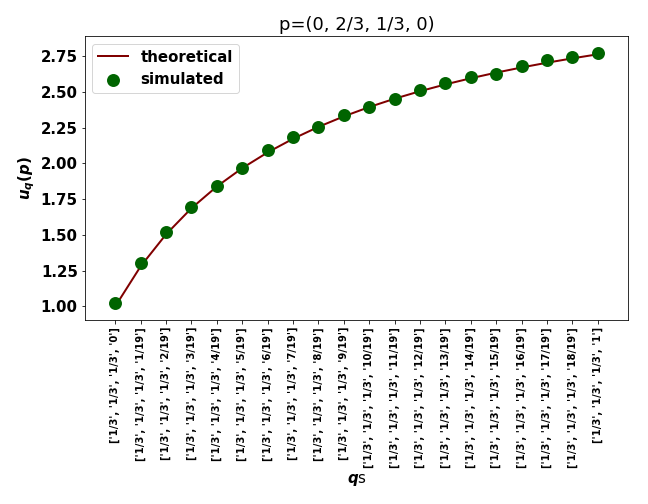
\includegraphics[width=\linewidth]{img/validation_img_two.png}
    \end{subfigure}
    \begin{subfigure}{0.45\textwidth}
        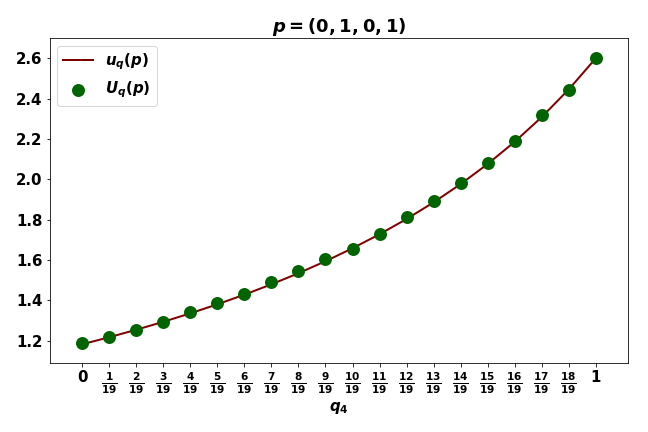
\includegraphics[width=\linewidth]{img/validation_img_three.png}
    \end{subfigure}
\end{center}
\caption{Differences between simulated and analytical results.}
\label{fig:analytical_simulated}
\end{figure}

Now that the analytical formulation has been validated in the following Sections
is used to explore bests responses in memory one strategies. Moreover, the new
formulation of Theorem~\ref{theorem:quadratic_form_u} allow us to retrieve a number
of theoretical results. These are also discussed in the next sections.

\section{Analytically Results}\label{section:analytical_results}

In the introduction a question was raised: which memory one strategy is the \textbf{best response}
against another memory one? This will be considered as an optimisation problem,
where a memory one strategy \(p\) wants to optimise it's utility \(u_q(p)\)
against an opponent \(q\). The decision variable is the vector \(p\) and the
solitary constrains \(p \in \R^4_{[0, 1]} \). The optimisation problem is
given by~(\ref{eq:mo_optimisation}).

\begin{equation}\label{eq:mo_optimisation}
\begin{aligned}
& \max_p: && \frac{\frac{1}{2}  p  Q  p^T + c^T p + a} 
                  {\frac{1}{2}  p  \bar{Q}  p^T + \bar{c}^T  p + \bar{a}}
\\
& \text{such that}: && \ p \in \R^4_{[0, 1]}.
\end{aligned}
\end{equation}

\subsection{Convexity}

This work is concerned with a fractional optimisation problem of quadratic forms.
Initially, the convexity, whether or not \(u_{q}(p)\) is concave~\cite{Gradshteyn2007},
is checked (concave because is a maximisation problem).

To test the hypothesis that \(u_q(p)\) is concave an empirical analysis
was performed using computer code. %TODO add the data generated
It was shown that there exists at least one point for which the definition of
concavity does not hold.

Several articles in fractional optimisation of quadratic forms that were non concave
can be found~\cite{Beck2009, Hongyan2014}. Though in these works both the numerator
and denominator of the fractional problem were concave. In~\cite{Anton2014} it is
stated that a quadratic form will be concave if and only if it's symmetric matrix is
negative semi definite. In Appendix, it is proved that neither the numerator or %TODO add appendix
the denominator of equation~(\ref{eq:optimisation_quadratic}) are concave.

\subsection{Best responses}\label{section:memory_one_analytical}

The non concavity of \(u(p)\) indicates multiple local optimal points. Thus we
are not searching a single optimal point but a set of candidate optimal points.
The aim is to introduce a compact way of constructing the candidate set. Once
the set is defined the point that maximises \(u(p)\) corresponds to the best
response strategy.

The problem considered is a bounded because \(p \in \R^4_{[0, 1]}\). Because of
this it is known that the candidate solutions will exist either at the boundaries
of the feasible solution space, either within that space. The method of Lagrange
Multipliers and Karush-Kuhn-Tucker conditions also agrees with this conclusion. %TODO add reference.
The Karush-Kuhn-Tucker conditions are used because our constrains are inequalities.

Thus the candidate solution set is constructed as follows:

\begin{itemize}
    \item any or all of \(p_1, p_2, p_3, p_4\) are \(\in {0, 1}\)
    \item the rest or all of \(p_1, p_2, p_3, p_4\) are given by the roots of \(\frac{du}{dp}\).
\end{itemize}

The derivative \(\frac{du}{dp}\) is given by,

\begin{equation}\label{eq:derivative_of_quadratic}
    \begin{aligned}
     \frac{du}{dp} & = && \frac{(  \frac{1}{2}p  Q  p^T + c p + a)'
      (  \frac{1}{2} p  \bar{Q}  p^T + \bar{c}  p + \bar{a}) - 
      (  \frac{1}{2} p  \bar{Q}  p^T + \bar{c}  p + \bar{a})'
      (  \frac{1}{2} p  Q  p^T + c p + a)}
      {(  \frac{1}{2} p  \bar{Q}  p^T + \bar{c}  p + \bar{a})^2} \\
      \\
    & = && \frac{(pQ + c) ( \frac{1}{2} p  \bar{Q}  p^T + \bar{c}  p + \bar{a}) 
    - (p\bar{Q} + \bar{c})( \frac{1}{2} p  Q  p^T + c p + a)}
      {( \frac{1}{2} p  \bar{Q}  p^T + \bar{c}  p + \bar{a})^2} \\
    \end{aligned}
\end{equation}

For equation~\ref{eq:derivative_of_quadratic} to be zero, the numerator must fall
to zero and the denominator can not nullified. Thus we conclude that the best
response of a memory one strategy in match is given by Lemma~\ref{lemma:memone_best_response}.

\begin{lemma}\label{lemma:memone_best_response}
    The optimal behaviour of a memory one strategy player \((p^*)\) against a
    given opponent \(q\) is given by:
    
    \[p^* = \textnormal{argmax}(u_q(p)), \ p \in S_q,\]
    
    where the set \(S_q\) is defined as 
    
    \[S_q = \{0, \bar{p}, 1 \}^4 \]
    
    where the vector \(\bar{p}\) is the vector for which the following conditions
    are true:
    
    {\small
    \begin{equation}\label{eq:derivative_numerator_condition}
        (pQ + c) ( \frac{1}{2} p  \bar{Q}  p^T + \bar{c}  p + \bar{a}) 
        - (p\bar{Q} + \bar{c})( \frac{1}{2} p  Q  p^T + c p + a) = 0
    \end{equation}}

    and

    {\small
    \begin{equation}
        \frac{1}{2} p  \bar{Q}  p^T + \bar{c}  p + \bar{a} \neq 0
    \end{equation}}

    Note that equation~\ref{eq:derivative_numerator_condition}  is a \(4-\)
    polynomial system of \(4\) variables. Each polynomial corresponds to a partial
    derivative of \(u_q(p)\).
\end{lemma}

A question that arises immediately after capturing best responses of memory one
strategies in pairwise interactions is: What is the optimal memory player against
multiple opponents, in a tournament environment. Let us consider a collection of
opponents: \(\{q^{(1)}, q^{(2)}, \dots, q^{(N)}\}\),  finding the optimal behaviour
is captured as:

\begin{equation}\label{eq:mo_tournament_optimisation}
\begin{aligned}
\max_p: & \ \frac{1}{N} \sum_{i=1} ^ {N} {u_q}^{(i)} (p) 
\\
st: & \ p \in \R_{[0, 1]} 
\end{aligned}
\end{equation}

where,

\begin{equation}\label{eq:tournament_utility}
    \frac{1}{N} \sum\limits_{i=1} ^ {N} {u_q}^{(i)} (p) = \frac{1}{N}
    \frac{\sum\limits_{i=1} ^ {N} (\frac{1}{2} pQ^{(i)} p^T + c^{(i)} p + a^ {(i)})
    \prod\limits_{\tiny\begin{array}{l} j=1 \\ j \neq i \end{array}} ^ 
    N (\frac{1}{2} p\bar{Q}^{(i)} p^T + \bar{c}^{(i)} p + \bar{a}^ {(i)})}
    {\prod\limits_{i=1} ^ N (\frac{1}{2} p\bar{Q}^{(i)} p^T + \bar{c}^{(i)} p + \bar{a}^ {(i)})}.
\end{equation}

Thus, we are optimising against the average utility over the set of opponents.
Note that the best response can not be captured by optimising against the mean
opponent. Thus, 

\begin{equation}\label{eq:tournament_hypothesis}
    \max_p \frac{1}{N} \sum_{i=1} ^ {N} {u_q}^{(i)} (p) \neq \max_p
      u_{\frac {1}{N} \sum\limits_{i=1} ^ N q^{(i)}}(p).
\end{equation}

A number of numerical experiments have been performed for cases where \(p=(p, p, p, p\)
and \(p= (p_1, p_2, p_1, p_2)\). This was done in order to compare the right hand
side of equation~(\ref{eq:tournament_hypothesis}) to the left. The fact that
equation~(\ref{eq:tournament_hypothesis}) holds is evident by Figure~\ref{fig:hypothesis}.

\begin{figure}[!htbp]
    \begin{center}
        \begin{subfigure}{0.45\textwidth}
            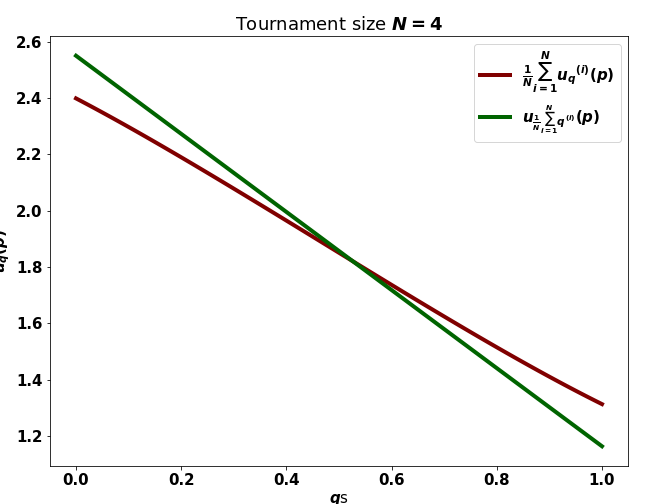
\includegraphics[width=\linewidth]{img/mean_vs_average.png}
        \end{subfigure}
        \begin{subfigure}{0.45\textwidth}
            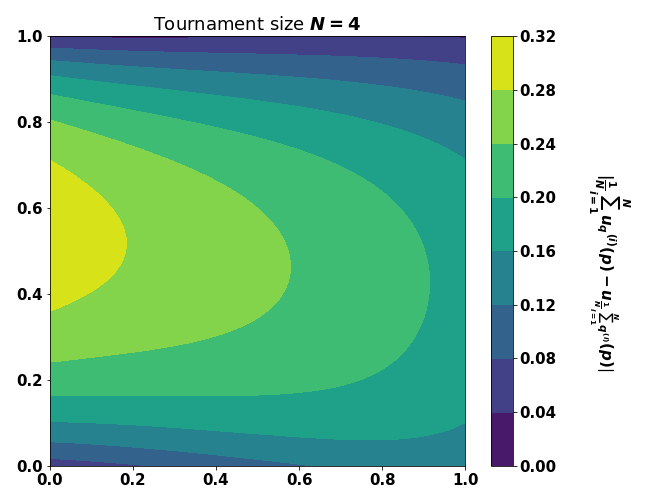
\includegraphics[width=\linewidth]{img/mean_vs_average_two.png}
        \end{subfigure}
    \end{center}
    \caption{Hypothesis.}
    \label{fig:hypothesis}
\end{figure}

A similar approach to the one considered for problem~\ref{eq:mo_optimisation} needs
to be used for problem~\ref{eq:mo_tournament_optimisation} as well. The candidate
solutions set would be constructed by considering the bounds of the feasible space
and the roots of the derivative \(\frac{d}{dp} \frac{1}{N} \sum\limits_{i=1} ^ {N} {u_q}^{(i)} (p)\).
The derivative is given by,

{\scriptsize
\begin{align}\label{eq:mo_tournament_derivative}
    \frac{d}{dp} \frac{1}{N} \sum\limits_{i=1} ^ {N} {u_q}^{(i)} (p) & = \nonumber \\
    & =\frac{
    (\sum\limits_{i=1} ^ {N} Q_{N}^{(i)'} \prod\limits_{\tiny\begin{array}{l} j=1 \\ j \neq i \end{array}} ^ N Q_{D}^{(i)}
    + \sum\limits_{i=1} ^ {N} Q_{D}^{(i)'} \sum\limits_{\tiny\begin{array}{l} j=1 \\ j \neq i \end{array}} ^ {N} Q_{N}^{(i)}
    \prod\limits_{\tiny\begin{array}{l} l=1 \\ l \neq i \ \\ l \neq j \end{array}} ^ N Q_{D}^{(i)}) \times
    \prod\limits_{i=1} ^ N Q_{D}^{(i)} - (\sum\limits_{i=1} ^ {N} Q_{D}^{(i)'}
    \prod\limits_{\tiny\begin{array}{l} j=1 \\ j \neq i \end{array}} ^ N Q_{D}^{(i)}) \times 
    (\sum\limits_{i=1} ^ {N} Q_{N}^{(i)} \prod\limits_{\tiny\begin{array}{l} j=1 \\ j \neq i \end{array}} ^ N Q_{D}^{(i)})}
    {(\prod\limits_{i=1} ^ N Q_{D}^{(i)})^{2}}
\end{align}
}
where,

\begin{align*}
    Q_{N}^{(i) } & = \frac{1}{2} pQ^{(i)} p^T + c^{(i)} p + a^ {(i)}, \\
    Q_{N}^{(i)'} & =  pQ^{(i)} + c^{(i)}, \\
    Q_{D}^{(i) } & = \frac{1}{2} p\bar{Q}^{(i)} p^T + \bar{c}^{(i)} p + \bar{a}^ {(i)}, \\
    Q_{D}^{(i)'} & =  p\bar{Q}^{(i)} + \bar{c}^{(i)}. \\
\end{align*}

Extracting the roots of equation's~(\ref{eq:mo_tournament_derivative}) numerator
is not an easy task. This also applied to equation~(\ref{eq:derivative_numerator_condition}).
Both equations are a system of \(4\) polynomials and the degree of the polynomials
is gradually increasing every time an extra opponent is taken into account.

Because of that no further analytical consideration is given to problems~\ref{eq:mo_optimisation}
and~\ref{eq:mo_tournament_optimisation}. Instead both best responses of memory one
strategies, pairwise and in multi interactions, will be solved using numerical
methods. The methods are their results are discussed in the following Section.

Though best responses can no longer be explored in an exact analytical way
there are still many advantages by the formulation of Theorem~\ref{theorem:quadratic_form_u}.
In the following subsections several theoretical results and exact ways of identifying
best responses in constrained versions of problem~\ref{eq:mo_tournament_optimisation} are presented.
Moreover, the robustness of defection in specific interactions is investigated.

\subsection{Purely random}\label{section:purely_analytical}

The first constrained problem to be explored is that of the purely random strategies.
Purely random strategies are a set of memory one strategies where the transition
probabilities of each state are the same. The optimisation problem of (\ref{eq:mo_optimisation})
now has an extra constraint and is re written as,

\begin{equation}\label{eq:random_optimisation}
\begin{aligned}
\max_p: & \ \frac{1}{N} \sum_{i=1} ^ {N} {u_q}^{(i)} (p) 
\\
\text{such that}: & \ 0 \leq p \leq 1 \\
                  & p_1 = p_2 = p_3 = p_4 = p.
\end{aligned}
\end{equation}

Due to the additional constrain, \(\sum\limits_{i=1} ^ {N} {u_q}^{(i)} (p) \) is now a function of a single
variable \(p\) and it can be handled analytically. To construct the set of candidate
solutions a similar approach as the one described in previous sections is used. Thus:

\begin{itemize}
    \item either \(p\) is \(\in {0, 1}\)
    \item or \(p\) is given by the roots of \(\frac{d \sum\limits_{i=1} ^ {N} {u_q}^{(i)} (p)}{dp}\).
\end{itemize}

The roots of the derivative are given by nullifying the numerator of the derivative.
It has been proved, Appendix, that the degree of the numerator does not exceed
\(2 N\) where \(N\) is the number of opponents. Thus there are \(2N\) possible
roots in the feasible space. These results are summarized by Lemma~\ref{lemma:purely_optimisation}.

\begin{lemma}[Optimisation of purely random player in a tournament]
    \label{lemma:purely_optimisation}
    The optimal behaviour of a \textbf{purely random} player \((p, p, p, p)\)
    in an \(N-\)memory one player tournament, \(\{q_{(1)}, q_{(2)} \dots,q_{(N)} \}
    \) is given by:
    
    \[p^* = \textnormal{argmax}(\sum_{i=1} ^ {N} {u_q}^{(i)} (p) ), \ p \in S_{q(i)},\]
    
    where the set \(S_{q}\) is defined as:
    
    \[S_{q} = \{0, \lambda_i, 1\},\text{ for } i \in [1, 2N].\]

    Note that \(\lambda_i\) are the eigenvalues of the companion matrix corresponding
    to the numerator of \[\frac{d}{dp} \sum_{i=1} ^ {N} {u_q}^{(i)} (p)\]

    and \(\lambda_i\) are such that the denominator is not nullified.
    \end{lemma}

To compute the roots of the polynomial the algorithm used is that of computing the
eigenvalues of the corresponding companion matrix. The algorithm is presented
and discussed in~\cite{Edelman1995}.

Furthermore, for the case of the purely random players two more theoretical results
are discussed. These are the cases where:

\begin{itemize}
    \item the opponent has manage to make a random player indifferent
    \item the best behaviour is a pure strategy.
\end{itemize}

There is importance in both results. Initially, being indifferent refers to our
actions no having any effects on the match. Thus our behaviour can not be optimised.
Secondly, by a pure strategy we are referring to the edge cases, behaving as a
defector or a cooperator. In in those case it is know that \(p^*\) is \(\in {0, 1}\).
The results are given equivalently by Lemmas~\ref{lemma:constant} and~\ref{lemma:linear}
and they are respective to the actions of the opponent.

\begin{lemma}\label{lemma:constant}
    A given memory one player, \((q_1, q_2, q_3, q_4)\), makes a \textbf{purely
    random} player, \((p, p, p, p)\), indifferent if and only if, 
    \(-q_1 + q_2 + 2q_3 - 2q_4 = 0 \) and 
    \((q_2 - q_4 - 1)(q_1 - 2q_2 - 5q_3 + 7q_4 + 1) -(q_2 - 5q_4 - 1)(q_1 - q_2 - q_3 + q_4) = 0 \).
\end{lemma}

\begin{lemma}\label{lemma:linear}
    Against a memory one player, \((q_1, q_2, q_3, q_4)\), a \textbf{purely random}
    player would always play a pure strategy if and only if
    \((q_{1}q_{4} - q_{2} q_{3} + q_{3} - q_{4}) (4 q_{1} - 3 q_{2} - 4 q_{3} + 3 
    q_{4} - 1) = 0\).
\end{lemma}

Figure~\ref{fig:purely_lemmas} illustrates that conditions given by Lemma
\ref{lemma:constant} and~\ref{lemma:linear} capture the behaviour as described.

\begin{figure}[!htbp]
    \begin{center}
        \begin{subfigure}{0.45\textwidth}
            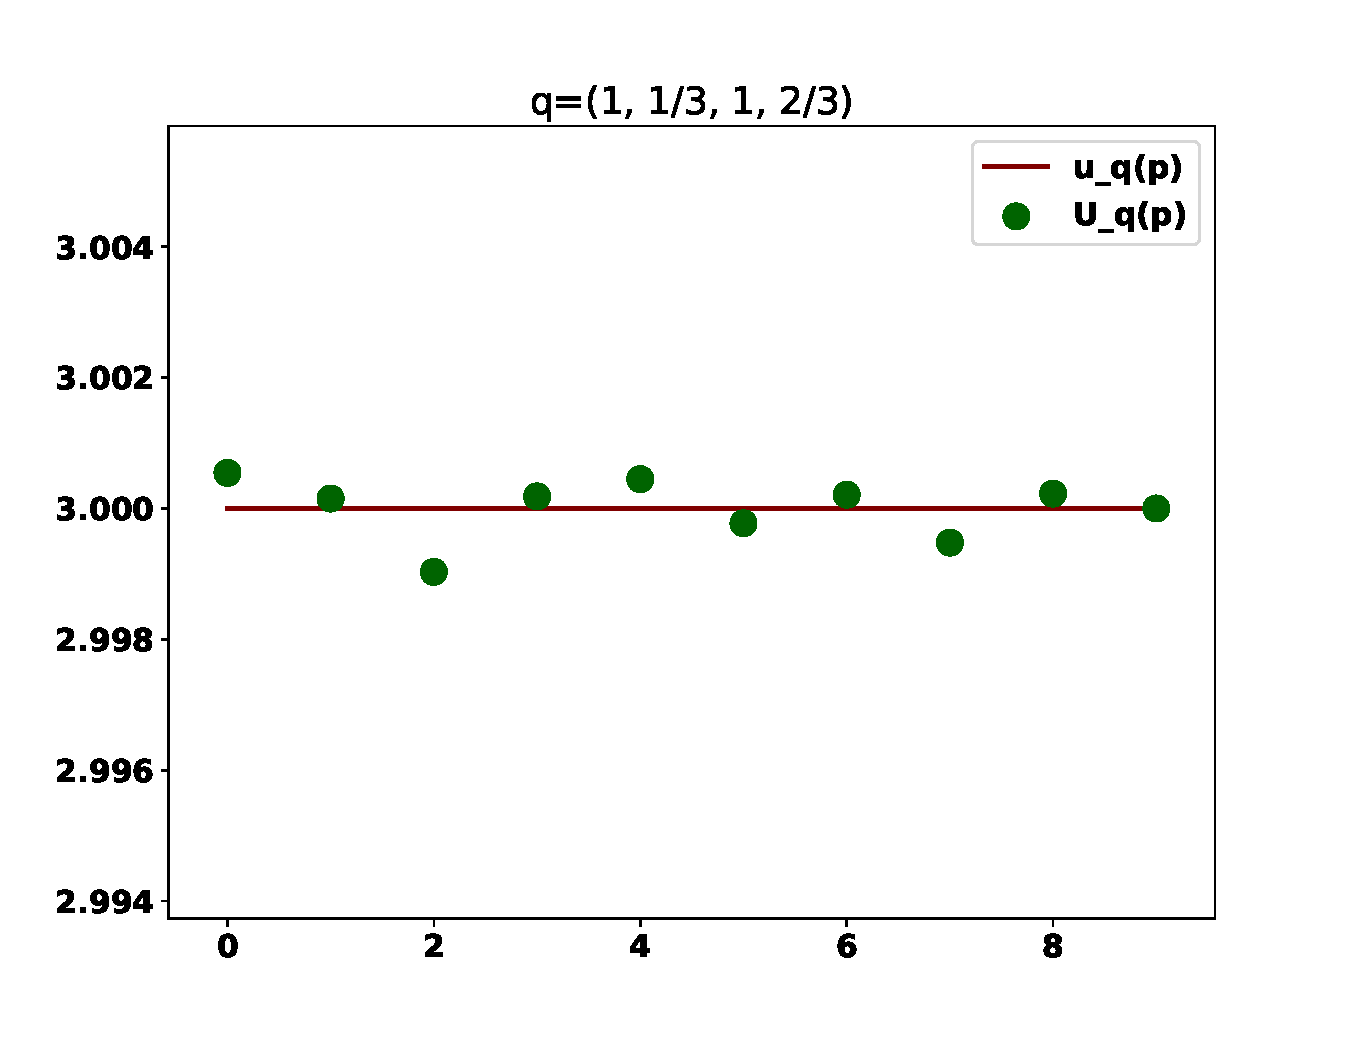
\includegraphics[width=\linewidth]{img/constant}
        \end{subfigure}
        \begin{subfigure}{0.45\textwidth}
            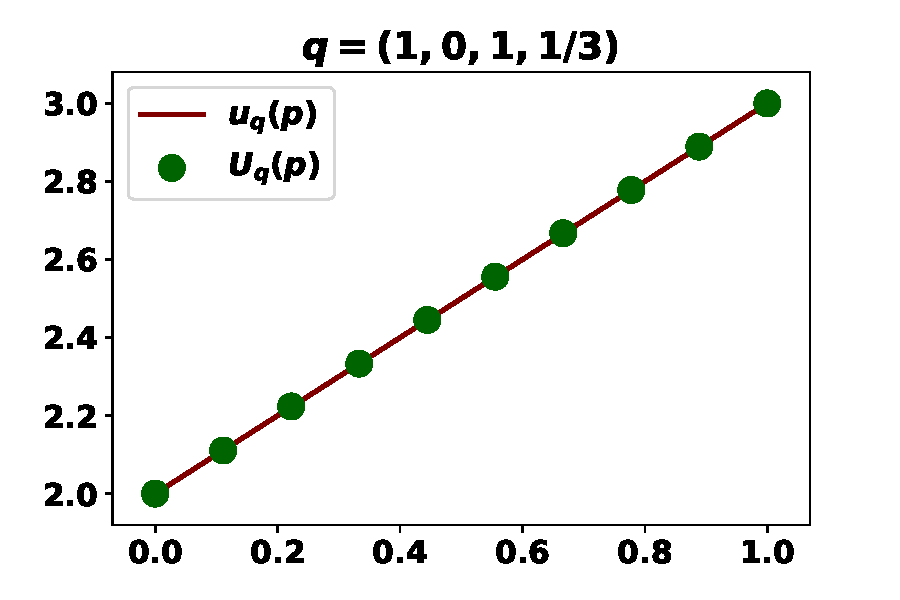
\includegraphics[width=\linewidth]{img/linear}
        \end{subfigure}
    \end{center}
    \caption{Proof of concept for Lemmas~\ref{lemma:constant},~\ref{lemma:linear}.}
    \label{fig:purely_lemmas}
\end{figure}


\subsection{Reactive Strategies}\label{section:reactive_analytical}

The next constrained case considered here is that of the reactive strategies.
Reactive strategies are a set of memory one strategies where they only take into
account the opponent's previous moves. As described in Section~\ref{section:introduction}
Tit for Tat is a reactive strategy. The optimisation problem of (\ref{eq:mo_optimisation})
now has an extra constraint and is re written as,

\begin{equation}\label{eq:random_optimisation}
\begin{aligned}
\max_p: & \ u_q(p)
\\
\text{such that}: & \ p_1 = p_3 \text{ and } p_2 = p_4\\
    & \ 0 \leq p_1, p_2 \leq 1.
\end{aligned}
\end{equation}

Reactive strategies allow us to study \(u_p\) as a function of two variables
\(p_1, p_2\). The candidate solution set can be constructed as follows:

\begin{itemize}
    \item \(p_1, p_2\) are \(\in \{0, 1\} ^ 2\)
    \item the rest or all of \(p_1, p_2\) are given by the roots of \(\frac{du}{dp}\).
\end{itemize}

Note that now,

\[\frac{du}{dp} = 0 \]

is now a system of 2 polynomials over 2 variables. Each polynomial is equivalent
to a partial derivative over \(p_1\) and \(p_2\). There are many methods that allow
us to solve that analytical. In this work we will be using resultant theory to
extract the roots.

The resultant is a symmetric function of the roots of the polynomials of a system
and it can be expressed as a polynomial in the coefficients of the polynomials.
The resultant will equal zero if and only if the system has at least one common
root. Thus, the resultant becomes very useful in identifying whether common roots exist.

In this work the Sylvester's resultant~\cite{Akritas1991} denoted as (\(R_S\))
is considered. The Sylvester's resultant is used to solve system of a single
variable. However, for a system of two variables we solve over one variable and
the second is kept as a coefficient. Thus we can find the roots of the equations
and that is why the resultant is often refereed to as the eliminator.

Thus the best response of a reactive strategy is given in very similar approach
as that described in Lemma~\ref{eq:mo_optimisation}. However now the partial derivatives can be
solved using an exact method. Note that for pairwise interactions the maximum degree
of the polynomials is equal to \(2N\), however the degree increases as opponents
are introduced.

\subsection{Stability of defection}

The final theoretical result explored is the stability of defection. Defection is
the dominant strategy in the one shot game and it can be proven to be an optimal
strategy in given environments. 

In this manuscript we try to provide a condition for when defection is the
best response. This will be done by considering equation~(\ref{eq:derivative_of_quadratic}).
Let equation~(\ref{eq:derivative_of_quadratic}) for \(p_0 = (0, 0, 0, 0)\) given by,


\begin{equation}\label{eq:derivative_of_quadratic_zero}
    \begin{aligned}
     \frac{du}{dp_0} & = && \frac{c \bar{a} - \bar{c}a}
      {\bar{a}^2} .\\
    \end{aligned}
\end{equation}

The numerator \(\bar{c}a - c\bar{a}\) is given by,

\[\input{tex/defection_matrix.txt}\]

and \(\bar{a} ^ 2 = (-q_2 + q_4 + 1) ^ 2\) which is always positive. In order
for defection to be the best response the derivative must have a negative
sign at the point \(p_0\). That means that the utility is only
decreasing after \(p_0\) and the points before are outside our feasible
space.

The sign of the derivative is given by the numerator, thus \(\bar{c}a - c\bar{a}\).
More specifically from equations,

\begin{equation}\label{eq:defection_condition_one}
    \input{tex/defection_condition_one.txt}
\end{equation}
\begin{equation}\label{eq:defection_condition_two}
    \input{tex/defection_condition_two.txt}
\end{equation}

Both signs of the partial derivatives must be negative in order for the overall
function to be decreasing, thus defection being the best response.
The signs of equations (\ref{eq:defection_condition_one}) and (\ref{eq:defection_condition_two})
vary. There are cases that they have the same sign and cases that they do not,
this is shown by numerical example summarized in Table~\ref{table:sign_of_derivative}.

\begin{table}[htbp]
\begin{center}
\begin{tabular}{cllllcc}
    \toprule
    {}& {} & {}& {}& {}&  equation(\ref{eq:defection_condition_one}) &  equation(\ref{eq:defection_condition_two}) \\
    \midrule
1 & \(q_1=\frac{3}{10}\),   & \(q_2=\frac{3}{20}\),  & \(q_3=\frac{13}{20}\), & \(q_4=\frac{7}{100}\)
&  + & + \\
2 & \(q_1=\frac{11}{25}\),  & \(q_2=\frac{3}{10}\),  & \(q_3=\frac{9}{10}\),  & \(q_4=\frac{1}{2}\)
&  - & - \\
3 & \(q_1=\frac{17}{20}\),  & \(q_2=\frac{3}{4}\),   & \(q_3=\frac{2}{5}\),   & \(q_4=\frac{1}{4}\)
&  - & + \\
4 & \(q_1=\frac{13}{88}\),  & \(q_2=\frac{21}{92}\),  & \(q_3=\frac{21}{26}\),  & \(q_4=\frac{20}{67}\)
&  + & - \\
    \bottomrule
\end{tabular}
\end{center}
\caption{Numerical examples of the derivative's sign.}
\label{table:sign_of_derivative}
\end{table}

Lets us consider a constrained version of the problem once again. Lets us
assume that the opponent is the  a reactive player \(q=(q_1, q_2, q_1, q_2)\).
By substituting \(q_3=q_1\) and \(q_4=q_2\) equations (\ref{eq:defection_condition_one})
and (\ref{eq:defection_condition_two}) are know re written as follow,

\[\left[\begin{matrix}- q_{2} \left(4 q_{1} - 5 q_{2} - 1\right)\\
\left(q_{2} - 1\right) \left(4 q_{1} - 5 q_{2} - 1\right)\end{matrix}\right]\]

The sign of both equations is now based on the same term,\(\left(4 q_{1} - 5 q_{2} - 1\right)\),
which is a term that can have both negative and positive values. This is shown
by Figure~\ref{fig:sign_against_reactive}. Following this the following result is retrieved,

\begin{figure}[htbp]
    \centering
    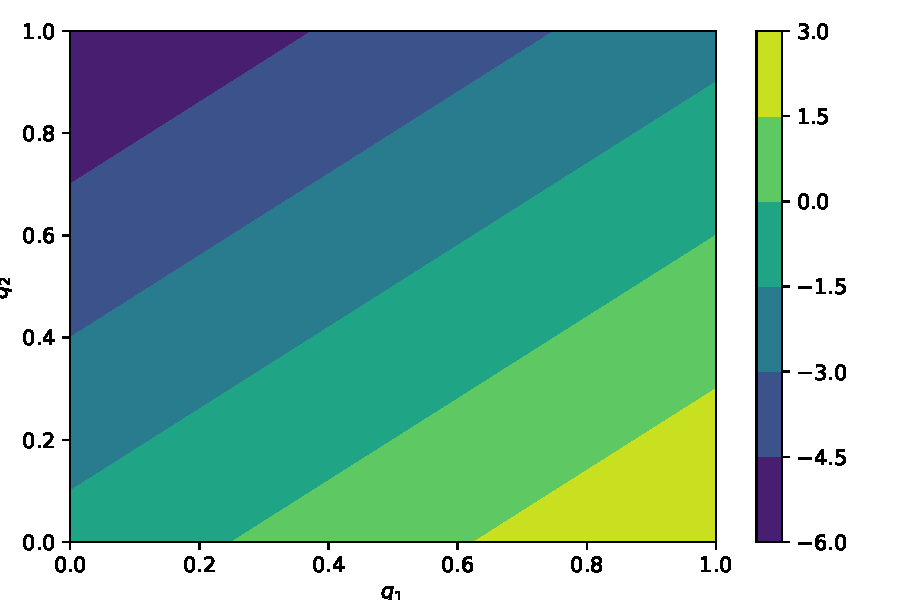
\includegraphics[width=0.45\linewidth]{img/sign_against_reactive.pdf}
      \caption{Sign of \(\left(4 q_{1} - 5 q_{2} - 1\right)\).}
      \label{fig:sign_against_reactive}
  \end{figure}

\begin{lemma}
Against a given reactive opponent \(q=(q_1, q_2, q_1, q_2)\) defection is said
to be stationary if and only if \(\left(4 q_{1} - 5 q_{2} - 1\right)\) is negative.
\end{lemma}

In tournaments the derivative~\ref{eq:derivative_of_quadratic} when we substitute
for \(p_0\) the equation is given by:
 
\begin{equation}
\sum_{i=1} ^ N (c^{(i)T} \bar{a}^{(i)} - \bar{c}^{(i)T} a^{(i)})
\prod\limits_{\tiny\begin{array}{l} j=1 \\ j \neq i \end{array}} ^ N (\bar{a}^{(i)})^2
\end{equation}

The product is know to be positive thus in order for defection to be stable
in a tournament falls down to a similar case the match one. Now the sum of
columns must be negative.

\section{Numerical Experiments}

In this section several analytical results of Section~\ref{section:analytical_results}
are validated using numerical experiments. Both methods and results are discussed.
Initially, numerical methods for best responses in the constrained versions of
the problem are presented. These further constrained problems taken into account
in this work were:

\begin{itemize}
    \item purely random strategies
    \item reactive strategies.
\end{itemize}

Moreover the answer to the questions discussed in Section~\ref{section:memory_one_analytical}
are answered via numerical algorithms. The question risen was identifying the best
response memory one strategy.

\subsection{Purely Random Strategies}

Best responses of purely random strategies were given by Lemma~\ref{lemma:purely_optimisation}
as presented in Section~\ref{section:purely_analytical}. Based on the results
Algorithm~\ref{algo:purely} is constructed to perform a number of numerical experiments
for pairwise and multi agent interactions.

\begin{algorithm}
    \setstretch{1.35}
    \caption{Best response algorithm for purely random strategies}\label{algo:purely}
    \begin{algorithmic}[1]
    \Procedure{Purely random search}{}
    \State $N \gets \text{number of opponets}$ 
    \State $S_q \gets \{0, 1\}$ 
    \State $u' \gets \frac{d\sum\limits_{i=1} ^ {N}u}{d\bar{p}}$ 
    \State $\frac{u_N}{u_D} \gets u'$ 
    \State $C(u_N) \gets \text{companion matrix of } u_N$
    \BState \emph{loop} $i=1 \text{ to } 2N$:
    \State $\lambda_i \gets \text{eigenvalue of } C(u_N)$
    \If {$u_D(\lambda_i) \neq 0$}
    \State $S_q \cup \lambda_i $.
    \EndIf
    \State \textbf{goto} \emph{loop}.
    \State \textbf{close};
    \State $p^* \gets \text{argmax}(\sum\limits_{i=1} ^ {N} u_{q^{(i)}} (p)), p \in S_q $.
    \EndProcedure
    \end{algorithmic}
    \end{algorithm}

The results of pairwise interactions are given by Figure~\ref{fig:purely_random_pairwise_results}.
There is it evident that the optimal behaviour has been captured by our search algorithm.
Moreover, the algorithm is also validated for tournament interactions, as shown
by Figure~\ref{fig:purely_random_tournament_results}.

\begin{figure}
    \centering
    \begin{subfigure}{0.45\textwidth}
        \centering
        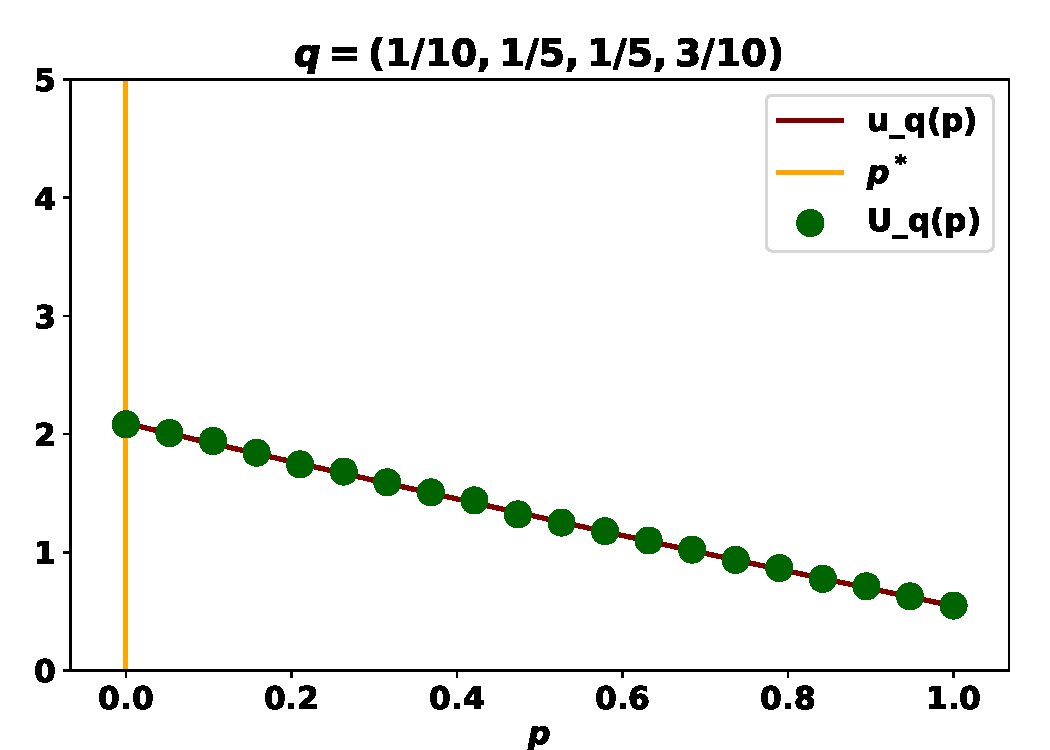
\includegraphics[width=.95\textwidth]{img/purely_random_match_one.pdf}
    \end{subfigure}
    \begin{subfigure}{0.45\textwidth}
        \centering
        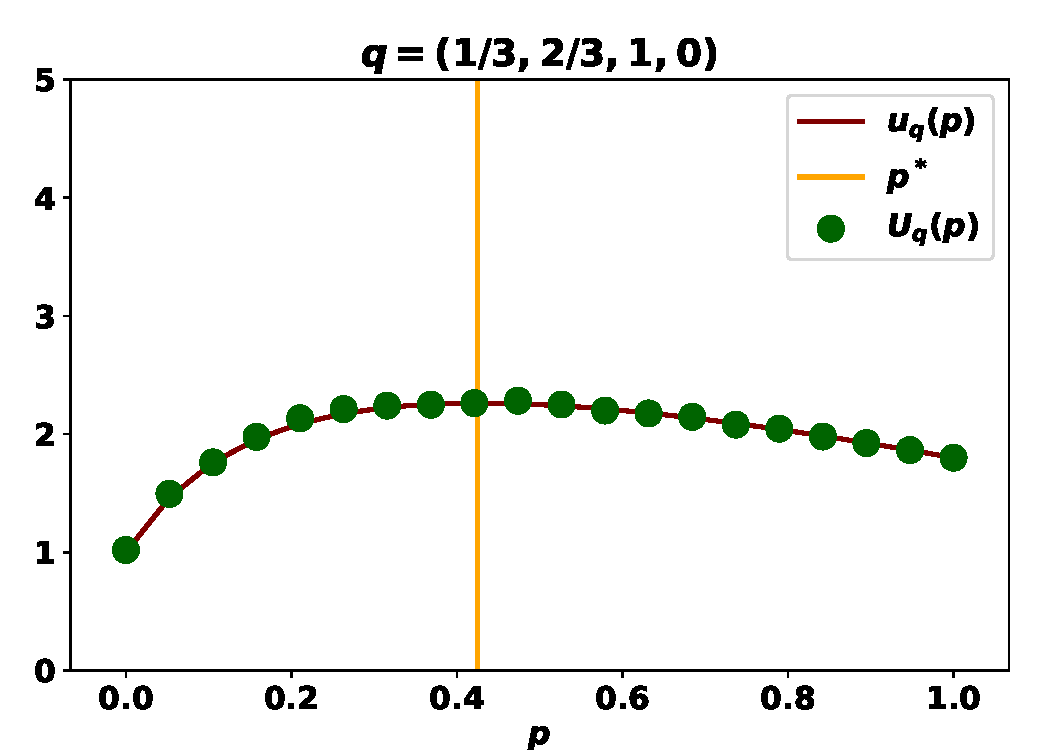
\includegraphics[width=.95\textwidth]{img/purely_random_match_two.pdf}
    \end{subfigure}
    \caption{Numerical experiments for Algorithm~\ref{algo:purely} for \(N=1\).}
    \label{fig:purely_random_pairwise_results}
\end{figure}

\begin{figure}
    \centering
    \begin{subfigure}{0.45\textwidth}
        \centering
        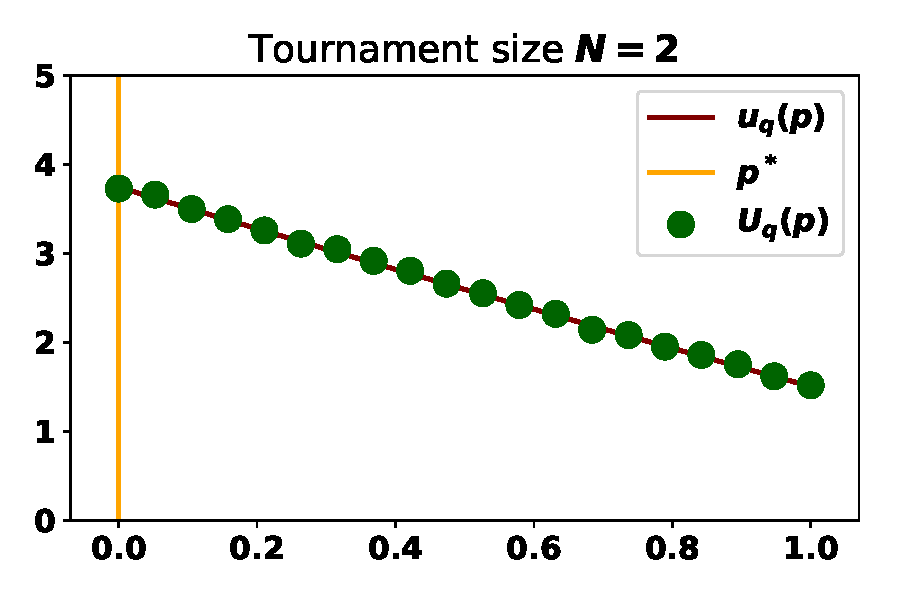
\includegraphics[width=.95\textwidth]{img/purely_random_tournament_one.pdf}
    \end{subfigure}
    \begin{subfigure}{0.45\textwidth}
        \centering
        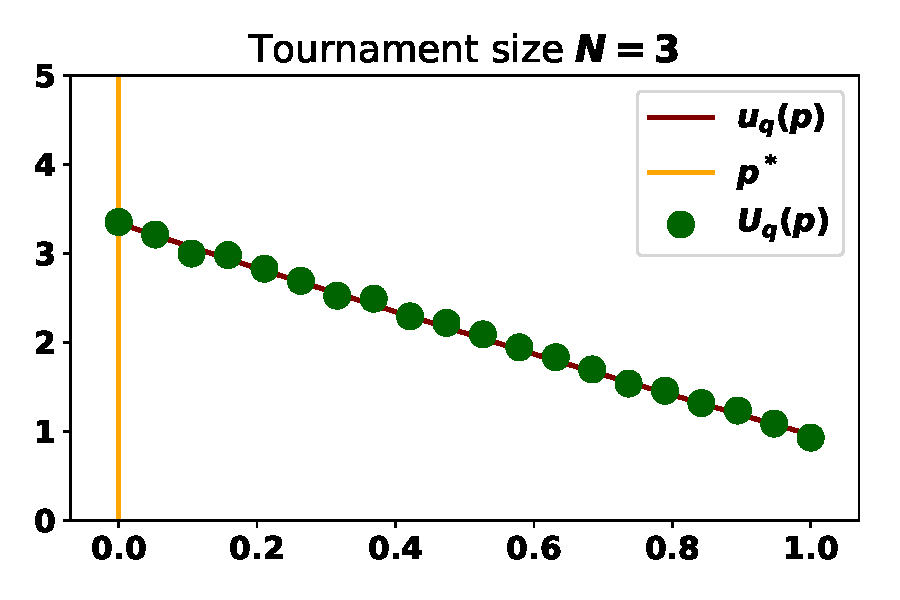
\includegraphics[width=.95\textwidth]{img/purely_random_tournament_two.pdf}
    \end{subfigure}
    \caption{Numerical experiments for Algorithm~\ref{algo:purely} for \(N>1\).}
    \label{fig:purely_random_tournament_results}
\end{figure}

\subsection{Reactive Strategies}

Best responses of reactive strategies have been discussed in Section~\ref{section:reactive_analytical}.
There it was stated that the field of resultant theory would be used to solve the
partial derivatives of the utility. As reminder, best responses in reactive
build upon Lemma~\ref{lemma:memone_best_response} however now condition
(\ref{eq:derivative_numerator_condition}) is a 2 polynomial system of 2 variables.

Based on the results Algorithm~\ref{algo:purely} is constructed to perform a number
of numerical experiments for pairwise and multi agent interactions.

\begin{algorithm}
    \setstretch{1.35}
    \caption{Best response algorithm for reactive strategies}\label{algo:reactive}
    \begin{algorithmic}[1]
    \Procedure{Reactive search}{}
    \State $N \gets \text{number of opponets}$ 
    \State $S_q \gets \{0, 1\} ^ 2$ 
    \State $u' \gets \frac{d\sum\limits_{i=1} ^ {N}u}{d\bar{p}}$ 
    \State $\frac{u_N}{u_D} \gets u'$ 
    \State $S(u_N, p_2) \gets \text{Sylvester's matrix for} p_2. \text{Coefficients are polynomials of } p_1$
    \State $R_S(S) \gets det(S)$
    \State $\text{roots}_{p_1} \gets p_1 \text{ for } det(M)_{p_1} = 0$
    \BState \emph{loop} $\text{root in roots}_{p_1}$:
    \State $\text{ system}(p_2) \gets u_N (root)$
    \State $\text{root}_{p_2} \cup {p_2} \text{ for } \text{system}(p_2) = 0$
    \If {$u_D((\text{root}, \text{root}_{p_2})) \neq 0$}
    \State $S_q \cup \{(\text{root}, \text{root}_{p_2})\}$
    \EndIf
    \State \textbf{goto} \emph{loop}.
    \State \textbf{close};
    \State $p^* \gets \text{argmax}(\sum\limits_{i=1} ^ {N} u_{q^{(i)}} (p)), p \in S_q$.
    \EndProcedure
    \end{algorithmic}
\end{algorithm}

Illustrated by Figure~\ref{fig:reactive_pairwise_results} are the results of the
numerical experiments for pairwise interactions. The results suggest that the best
response behaviour is captured by our algorithm.

\begin{figure}
    \centering
    \begin{subfigure}{0.45\textwidth}
        \centering
        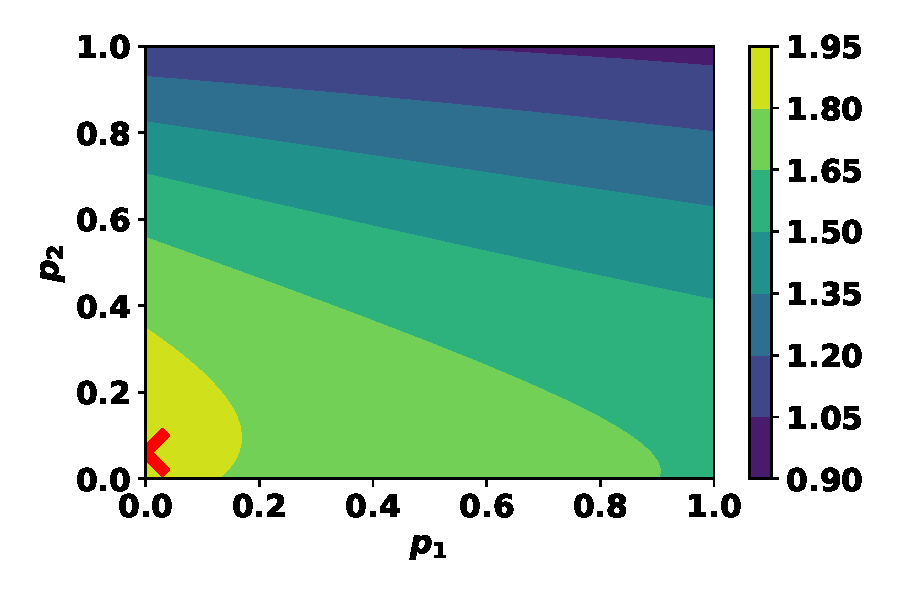
\includegraphics[width=.95\textwidth]{img/reactive_pairwise_one.pdf}
    \end{subfigure}
    \begin{subfigure}{0.45\textwidth}
        \centering
        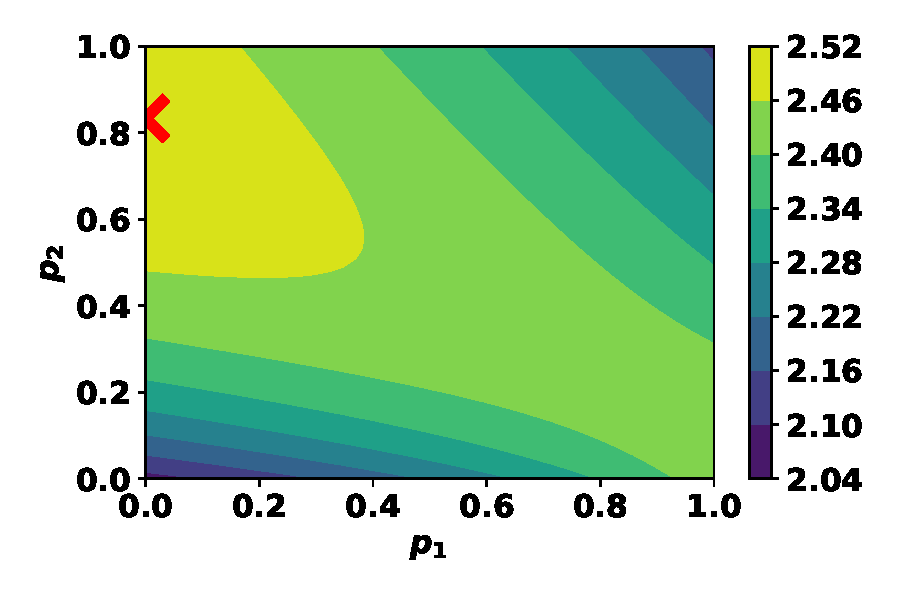
\includegraphics[width=.95\textwidth]{img/reactive_pairwise_two.pdf}
    \end{subfigure}
    \caption{Numerical experiments for Algorithm~\ref{algo:reactive} for \(N=1\).}
    \label{fig:reactive_pairwise_results}
\end{figure}

\subsection{Memory one strategies}

As discussed in section memory one strategies are explored numerically.
The algorithm used in order to maximise problem is bayesian optimisation.

\section{Limitation of memory}


\section{Discussion}

% Bibliography
\bibliographystyle{plain}
\bibliography{bibliography.bib}

\end{document}
